% Created by tikzDevice version 0.10.1 on 2017-05-27 09:46:04
% !TEX encoding = UTF-8 Unicode
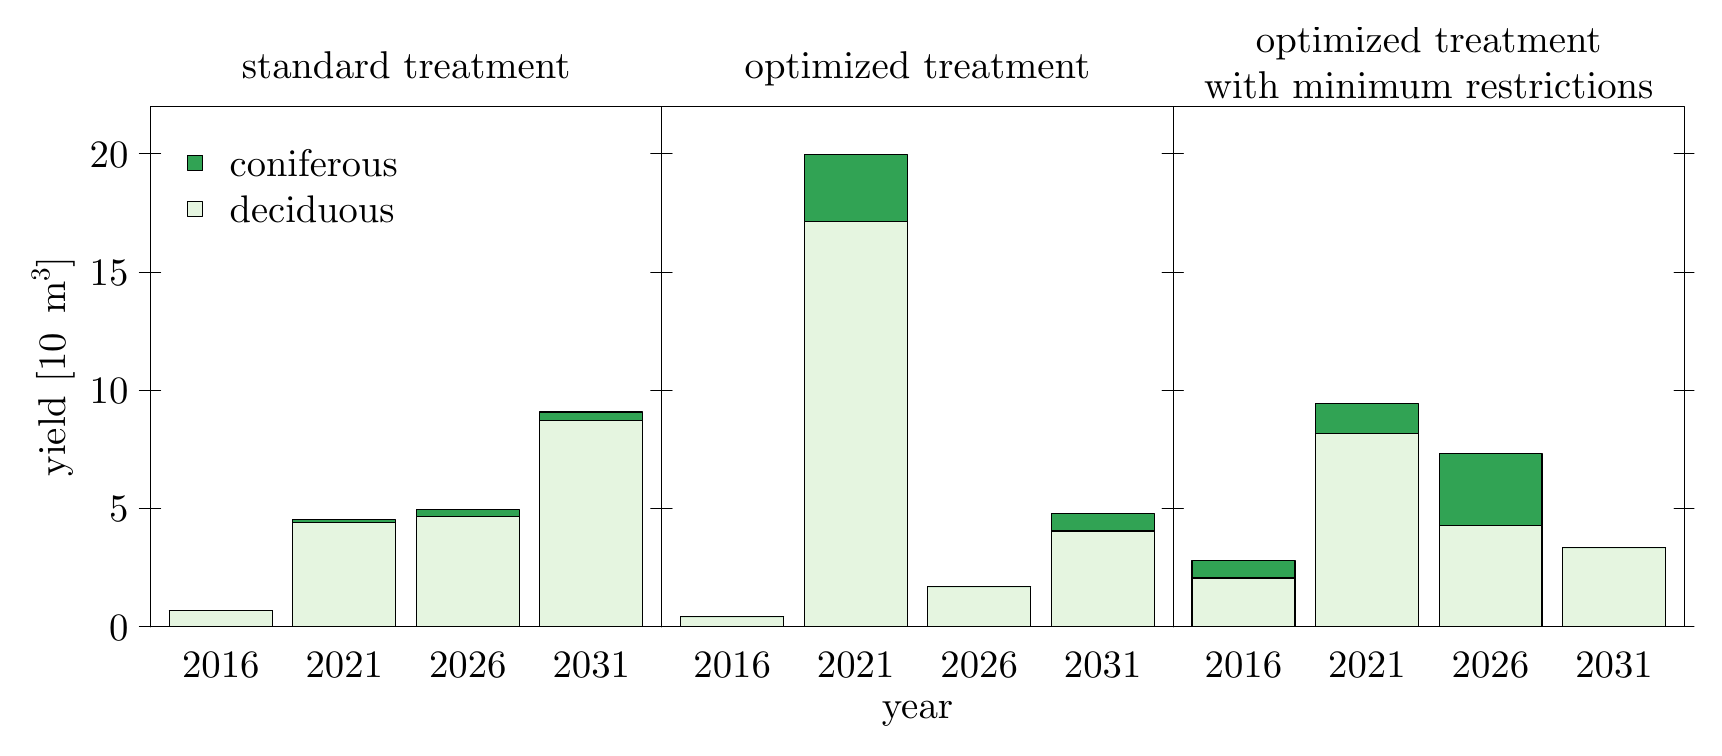
\begin{tikzpicture}[x=1pt,y=1pt]
\definecolor{fillColor}{RGB}{255,255,255}
\path[use as bounding box,fill=fillColor,fill opacity=0.00] (0,0) rectangle (602.23,252.94);
\begin{scope}
\path[clip] ( 44.35, 36.43) rectangle (229.12,224.43);
\definecolor{drawColor}{RGB}{0,0,0}
\definecolor{fillColor}{RGB}{229,245,224}

\path[draw=drawColor,line width= 0.4pt,line join=round,line cap=round,fill=fillColor] ( 51.20, 36.43) rectangle ( 88.39, 42.38);
\definecolor{fillColor}{RGB}{49,163,84}

\path[draw=drawColor,line width= 0.4pt,line join=round,line cap=round,fill=fillColor] ( 51.20, 42.38) rectangle ( 88.39, 42.38);
\definecolor{fillColor}{RGB}{229,245,224}

\path[draw=drawColor,line width= 0.4pt,line join=round,line cap=round,fill=fillColor] ( 95.83, 36.43) rectangle (133.02, 74.15);
\definecolor{fillColor}{RGB}{49,163,84}

\path[draw=drawColor,line width= 0.4pt,line join=round,line cap=round,fill=fillColor] ( 95.83, 74.15) rectangle (133.02, 75.13);
\definecolor{fillColor}{RGB}{229,245,224}

\path[draw=drawColor,line width= 0.4pt,line join=round,line cap=round,fill=fillColor] (140.46, 36.43) rectangle (177.65, 76.25);
\definecolor{fillColor}{RGB}{49,163,84}

\path[draw=drawColor,line width= 0.4pt,line join=round,line cap=round,fill=fillColor] (140.46, 76.25) rectangle (177.65, 78.97);
\definecolor{fillColor}{RGB}{229,245,224}

\path[draw=drawColor,line width= 0.4pt,line join=round,line cap=round,fill=fillColor] (185.09, 36.43) rectangle (222.28,110.88);
\definecolor{fillColor}{RGB}{49,163,84}

\path[draw=drawColor,line width= 0.4pt,line join=round,line cap=round,fill=fillColor] (185.09,110.88) rectangle (222.28,114.07);
\end{scope}
\begin{scope}
\path[clip] (  0.00,  0.00) rectangle (602.23,252.94);
\definecolor{drawColor}{RGB}{0,0,0}

\node[text=drawColor,anchor=base,inner sep=0pt, outer sep=0pt, scale=  1.40] at (136.74,234.45) {standard treatment};

\path[draw=drawColor,line width= 0.4pt,line join=round,line cap=round] ( 44.35, 36.43) -- ( 40.39, 36.43);

\path[draw=drawColor,line width= 0.4pt,line join=round,line cap=round] ( 44.35, 79.16) -- ( 40.39, 79.16);

\path[draw=drawColor,line width= 0.4pt,line join=round,line cap=round] ( 44.35,121.89) -- ( 40.39,121.89);

\path[draw=drawColor,line width= 0.4pt,line join=round,line cap=round] ( 44.35,164.61) -- ( 40.39,164.61);

\path[draw=drawColor,line width= 0.4pt,line join=round,line cap=round] ( 44.35,207.34) -- ( 40.39,207.34);

\node[text=drawColor,anchor=base east,inner sep=0pt, outer sep=0pt, scale=  1.40] at ( 36.43, 31.61) {0};

\node[text=drawColor,anchor=base east,inner sep=0pt, outer sep=0pt, scale=  1.40] at ( 36.43, 74.34) {5};

\node[text=drawColor,anchor=base east,inner sep=0pt, outer sep=0pt, scale=  1.40] at ( 36.43,117.07) {10};

\node[text=drawColor,anchor=base east,inner sep=0pt, outer sep=0pt, scale=  1.40] at ( 36.43,159.79) {15};

\node[text=drawColor,anchor=base east,inner sep=0pt, outer sep=0pt, scale=  1.40] at ( 36.43,202.52) {20};

\path[draw=drawColor,line width= 0.4pt,line join=round,line cap=round] ( 44.35, 36.43) -- ( 48.05, 36.43);

\path[draw=drawColor,line width= 0.4pt,line join=round,line cap=round] ( 44.35, 79.16) -- ( 48.05, 79.16);

\path[draw=drawColor,line width= 0.4pt,line join=round,line cap=round] ( 44.35,121.89) -- ( 48.05,121.89);

\path[draw=drawColor,line width= 0.4pt,line join=round,line cap=round] ( 44.35,164.61) -- ( 48.05,164.61);

\path[draw=drawColor,line width= 0.4pt,line join=round,line cap=round] ( 44.35,207.34) -- ( 48.05,207.34);

\node[text=drawColor,anchor=base,inner sep=0pt, outer sep=0pt, scale=  1.40] at ( 69.79, 18.22) {2016};

\node[text=drawColor,anchor=base,inner sep=0pt, outer sep=0pt, scale=  1.40] at (114.42, 18.22) {2021};

\node[text=drawColor,anchor=base,inner sep=0pt, outer sep=0pt, scale=  1.40] at (159.05, 18.22) {2026};

\node[text=drawColor,anchor=base,inner sep=0pt, outer sep=0pt, scale=  1.40] at (203.68, 18.22) {2031};

\node[text=drawColor,rotate= 90.00,anchor=base west,inner sep=0pt, outer sep=0pt, scale=  1.40] at ( 13.53, 90.85) {yield [10};

\node[text=drawColor,rotate= 90.00,anchor=base west,inner sep=0pt, outer sep=0pt, scale=  1.40] at ( 13.53,142.56) { };

\node[text=drawColor,rotate= 90.00,anchor=base west,inner sep=0pt, outer sep=0pt, scale=  1.40] at ( 13.53,149.56) {m};

\node[text=drawColor,rotate= 90.00,anchor=base west,inner sep=0pt, outer sep=0pt, scale=  0.98] at (  7.80,161.22) {3};

\node[text=drawColor,rotate= 90.00,anchor=base west,inner sep=0pt, outer sep=0pt, scale=  1.40] at ( 13.53,166.12) {]};
\end{scope}
\begin{scope}
\path[clip] ( 44.35, 36.43) rectangle (229.12,224.43);
\definecolor{drawColor}{RGB}{0,0,0}
\definecolor{fillColor}{RGB}{49,163,84}

\path[draw=drawColor,line width= 0.4pt,line join=round,line cap=round,fill=fillColor] ( 57.76,201.28) rectangle ( 63.29,206.80);
\definecolor{fillColor}{RGB}{229,245,224}

\path[draw=drawColor,line width= 0.4pt,line join=round,line cap=round,fill=fillColor] ( 57.76,184.65) rectangle ( 63.29,190.17);

\node[text=drawColor,anchor=base west,inner sep=0pt, outer sep=0pt, scale=  1.39] at ( 73.00,199.27) {coniferous};

\node[text=drawColor,anchor=base west,inner sep=0pt, outer sep=0pt, scale=  1.39] at ( 73.00,182.64) {deciduous};
\end{scope}
\begin{scope}
\path[clip] (  0.00,  0.00) rectangle (602.23,252.94);
\definecolor{drawColor}{RGB}{0,0,0}

\path[draw=drawColor,line width= 0.4pt,line join=round,line cap=round] ( 44.35, 36.43) --
	(229.12, 36.43) --
	(229.12,224.43) --
	( 44.35,224.43) --
	( 44.35, 36.43);
\end{scope}
\begin{scope}
\path[clip] (229.12, 36.43) rectangle (413.89,224.43);
\definecolor{drawColor}{RGB}{0,0,0}
\definecolor{fillColor}{RGB}{229,245,224}

\path[draw=drawColor,line width= 0.4pt,line join=round,line cap=round,fill=fillColor] (235.97, 36.43) rectangle (273.16, 40.04);
\definecolor{fillColor}{RGB}{49,163,84}

\path[draw=drawColor,line width= 0.4pt,line join=round,line cap=round,fill=fillColor] (235.97, 40.04) rectangle (273.16, 40.04);
\definecolor{fillColor}{RGB}{229,245,224}

\path[draw=drawColor,line width= 0.4pt,line join=round,line cap=round,fill=fillColor] (280.60, 36.43) rectangle (317.79,182.76);
\definecolor{fillColor}{RGB}{49,163,84}

\path[draw=drawColor,line width= 0.4pt,line join=round,line cap=round,fill=fillColor] (280.60,182.76) rectangle (317.79,207.06);
\definecolor{fillColor}{RGB}{229,245,224}

\path[draw=drawColor,line width= 0.4pt,line join=round,line cap=round,fill=fillColor] (325.23, 36.43) rectangle (362.42, 50.87);
\definecolor{fillColor}{RGB}{49,163,84}

\path[draw=drawColor,line width= 0.4pt,line join=round,line cap=round,fill=fillColor] (325.23, 50.87) rectangle (362.42, 50.87);
\definecolor{fillColor}{RGB}{229,245,224}

\path[draw=drawColor,line width= 0.4pt,line join=round,line cap=round,fill=fillColor] (369.86, 36.43) rectangle (407.05, 71.06);
\definecolor{fillColor}{RGB}{49,163,84}

\path[draw=drawColor,line width= 0.4pt,line join=round,line cap=round,fill=fillColor] (369.86, 71.06) rectangle (407.05, 77.32);
\end{scope}
\begin{scope}
\path[clip] (  0.00,  0.00) rectangle (602.23,252.94);
\definecolor{drawColor}{RGB}{0,0,0}

\path[draw=drawColor,line width= 0.4pt,line join=round,line cap=round] (229.12, 36.43) -- (225.16, 36.43);

\path[draw=drawColor,line width= 0.4pt,line join=round,line cap=round] (229.12, 79.16) -- (225.16, 79.16);

\path[draw=drawColor,line width= 0.4pt,line join=round,line cap=round] (229.12,121.89) -- (225.16,121.89);

\path[draw=drawColor,line width= 0.4pt,line join=round,line cap=round] (229.12,164.61) -- (225.16,164.61);

\path[draw=drawColor,line width= 0.4pt,line join=round,line cap=round] (229.12,207.34) -- (225.16,207.34);

\path[draw=drawColor,line width= 0.4pt,line join=round,line cap=round] (229.12, 36.43) -- (232.82, 36.43);

\path[draw=drawColor,line width= 0.4pt,line join=round,line cap=round] (229.12, 79.16) -- (232.82, 79.16);

\path[draw=drawColor,line width= 0.4pt,line join=round,line cap=round] (229.12,121.89) -- (232.82,121.89);

\path[draw=drawColor,line width= 0.4pt,line join=round,line cap=round] (229.12,164.61) -- (232.82,164.61);

\path[draw=drawColor,line width= 0.4pt,line join=round,line cap=round] (229.12,207.34) -- (232.82,207.34);

\node[text=drawColor,anchor=base,inner sep=0pt, outer sep=0pt, scale=  1.40] at (254.56, 18.22) {2016};

\node[text=drawColor,anchor=base,inner sep=0pt, outer sep=0pt, scale=  1.40] at (299.19, 18.22) {2021};

\node[text=drawColor,anchor=base,inner sep=0pt, outer sep=0pt, scale=  1.40] at (343.82, 18.22) {2026};

\node[text=drawColor,anchor=base,inner sep=0pt, outer sep=0pt, scale=  1.40] at (388.45, 18.22) {2031};

\path[draw=drawColor,line width= 0.4pt,line join=round,line cap=round] (229.12, 36.43) --
	(413.89, 36.43) --
	(413.89,224.43) --
	(229.12,224.43) --
	(229.12, 36.43);

\node[text=drawColor,anchor=base,inner sep=0pt, outer sep=0pt, scale=  1.40] at (321.51,234.45) {optimized treatment};

\node[text=drawColor,anchor=base,inner sep=0pt, outer sep=0pt, scale=  1.40] at (321.51,  3.17) {year};
\end{scope}
\begin{scope}
\path[clip] (413.89, 36.43) rectangle (598.66,224.43);
\definecolor{drawColor}{RGB}{0,0,0}
\definecolor{fillColor}{RGB}{229,245,224}

\path[draw=drawColor,line width= 0.4pt,line join=round,line cap=round,fill=fillColor] (420.74, 36.43) rectangle (457.93, 54.09);
\definecolor{fillColor}{RGB}{49,163,84}

\path[draw=drawColor,line width= 0.4pt,line join=round,line cap=round,fill=fillColor] (420.74, 54.09) rectangle (457.93, 60.27);
\definecolor{fillColor}{RGB}{229,245,224}

\path[draw=drawColor,line width= 0.4pt,line join=round,line cap=round,fill=fillColor] (465.37, 36.43) rectangle (502.56,106.16);
\definecolor{fillColor}{RGB}{49,163,84}

\path[draw=drawColor,line width= 0.4pt,line join=round,line cap=round,fill=fillColor] (465.37,106.16) rectangle (502.56,117.07);
\definecolor{fillColor}{RGB}{229,245,224}

\path[draw=drawColor,line width= 0.4pt,line join=round,line cap=round,fill=fillColor] (510.00, 36.43) rectangle (547.19, 73.06);
\definecolor{fillColor}{RGB}{49,163,84}

\path[draw=drawColor,line width= 0.4pt,line join=round,line cap=round,fill=fillColor] (510.00, 73.06) rectangle (547.19, 99.15);
\definecolor{fillColor}{RGB}{229,245,224}

\path[draw=drawColor,line width= 0.4pt,line join=round,line cap=round,fill=fillColor] (554.63, 36.43) rectangle (591.82, 64.94);
\definecolor{fillColor}{RGB}{49,163,84}

\path[draw=drawColor,line width= 0.4pt,line join=round,line cap=round,fill=fillColor] (554.63, 64.94) rectangle (591.82, 64.94);
\end{scope}
\begin{scope}
\path[clip] (  0.00,  0.00) rectangle (602.23,252.94);
\definecolor{drawColor}{RGB}{0,0,0}

\path[draw=drawColor,line width= 0.4pt,line join=round,line cap=round] (413.89, 36.43) -- (409.93, 36.43);

\path[draw=drawColor,line width= 0.4pt,line join=round,line cap=round] (413.89, 79.16) -- (409.93, 79.16);

\path[draw=drawColor,line width= 0.4pt,line join=round,line cap=round] (413.89,121.89) -- (409.93,121.89);

\path[draw=drawColor,line width= 0.4pt,line join=round,line cap=round] (413.89,164.61) -- (409.93,164.61);

\path[draw=drawColor,line width= 0.4pt,line join=round,line cap=round] (413.89,207.34) -- (409.93,207.34);

\path[draw=drawColor,line width= 0.4pt,line join=round,line cap=round] (413.89, 36.43) -- (417.59, 36.43);

\path[draw=drawColor,line width= 0.4pt,line join=round,line cap=round] (413.89, 79.16) -- (417.59, 79.16);

\path[draw=drawColor,line width= 0.4pt,line join=round,line cap=round] (413.89,121.89) -- (417.59,121.89);

\path[draw=drawColor,line width= 0.4pt,line join=round,line cap=round] (413.89,164.61) -- (417.59,164.61);

\path[draw=drawColor,line width= 0.4pt,line join=round,line cap=round] (413.89,207.34) -- (417.59,207.34);

\path[draw=drawColor,line width= 0.4pt,line join=round,line cap=round] (598.66, 36.43) -- (602.23, 36.43);

\path[draw=drawColor,line width= 0.4pt,line join=round,line cap=round] (598.66, 79.16) -- (602.23, 79.16);

\path[draw=drawColor,line width= 0.4pt,line join=round,line cap=round] (598.66,121.89) -- (602.23,121.89);

\path[draw=drawColor,line width= 0.4pt,line join=round,line cap=round] (598.66,164.61) -- (602.23,164.61);

\path[draw=drawColor,line width= 0.4pt,line join=round,line cap=round] (598.66,207.34) -- (602.23,207.34);

\path[draw=drawColor,line width= 0.4pt,line join=round,line cap=round] (598.66, 36.43) -- (594.97, 36.43);

\path[draw=drawColor,line width= 0.4pt,line join=round,line cap=round] (598.66, 79.16) -- (594.97, 79.16);

\path[draw=drawColor,line width= 0.4pt,line join=round,line cap=round] (598.66,121.89) -- (594.97,121.89);

\path[draw=drawColor,line width= 0.4pt,line join=round,line cap=round] (598.66,164.61) -- (594.97,164.61);

\path[draw=drawColor,line width= 0.4pt,line join=round,line cap=round] (598.66,207.34) -- (594.97,207.34);

\node[text=drawColor,anchor=base,inner sep=0pt, outer sep=0pt, scale=  1.40] at (439.33, 18.22) {2016};

\node[text=drawColor,anchor=base,inner sep=0pt, outer sep=0pt, scale=  1.40] at (483.96, 18.22) {2021};

\node[text=drawColor,anchor=base,inner sep=0pt, outer sep=0pt, scale=  1.40] at (528.59, 18.22) {2026};

\node[text=drawColor,anchor=base,inner sep=0pt, outer sep=0pt, scale=  1.40] at (573.22, 18.22) {2031};

\node[text=drawColor,anchor=base,inner sep=0pt, outer sep=0pt, scale=  1.40] at (506.28,244.09) {optimized treatment};

\node[text=drawColor,anchor=base,inner sep=0pt, outer sep=0pt, scale=  1.40] at (506.28,227.29) {with minimum restrictions};

\path[draw=drawColor,line width= 0.4pt,line join=round,line cap=round] (413.89, 36.43) --
	(598.66, 36.43) --
	(598.66,224.43) --
	(413.89,224.43) --
	(413.89, 36.43);
\end{scope}
\end{tikzpicture}
